\documentclass[border=6pt]{standalone}
\usepackage{tikz}
\usetikzlibrary{shapes.geometric, arrows.meta, positioning, calc}
\begin{document}
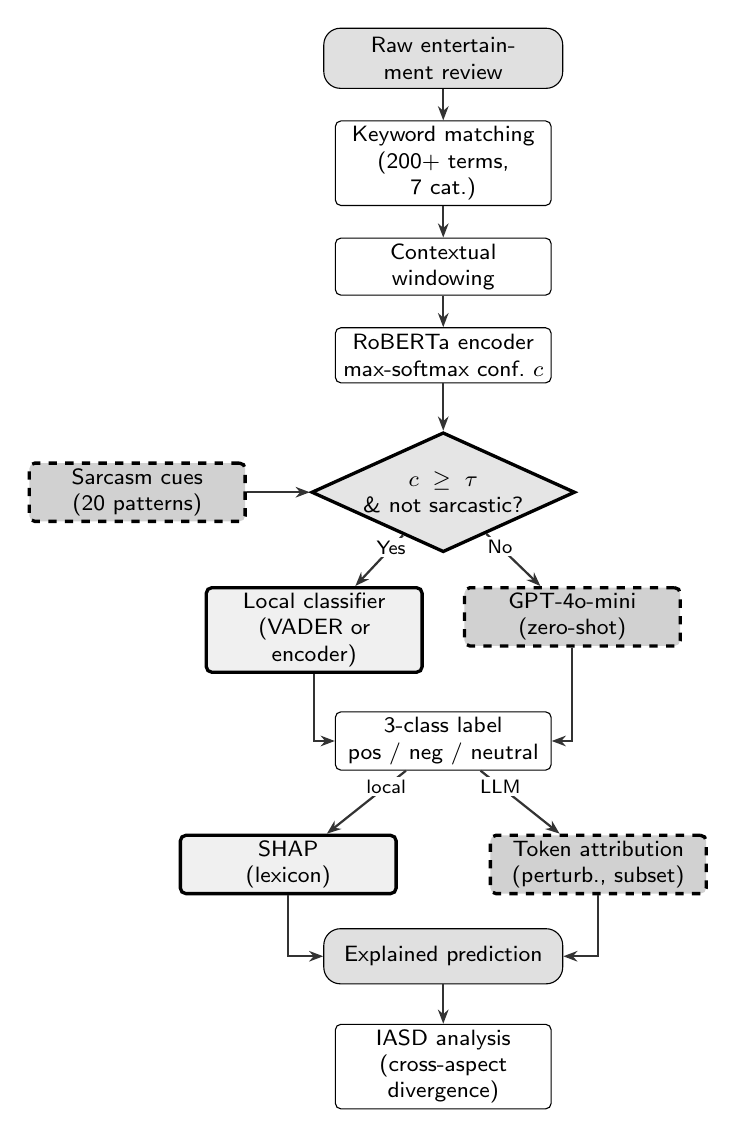
\begin{tikzpicture}[
  font=\sffamily\footnotesize, node distance=4mm and 8mm,
  box/.style={rectangle, rounded corners=2pt, draw=black, fill=white, text width=26mm, minimum height=7mm, align=center, inner sep=2pt},
  proc/.style={box},
  vader/.style={box, fill=black!6, draw=black, very thick},
  llm/.style={box, fill=black!18, draw=black, very thick, dashed},
  decision/.style={diamond, aspect=2.2, draw=black, very thick, fill=black!10, align=center, inner sep=0pt, text width=22mm},
  io/.style={rectangle, rounded corners=6pt, draw=black, fill=black!12, text width=28mm, minimum height=7mm, align=center},
  arr/.style={-{Stealth[length=1.8mm]}, draw=black!80, thick},
  lbl/.style={font=\sffamily\scriptsize, fill=white, inner sep=1pt}]
\node[io] (input) {Raw entertainment review};
\node[proc, below=of input] (extract) {Keyword matching\\(200+ terms, 7 cat.)};
\node[proc, below=of extract] (window) {Contextual windowing};
\node[proc, below=of window] (roberta) {RoBERTa encoder\\max-softmax conf.\ $c$};
\node[decision, below=6mm of roberta] (gate) {$c \ge \tau$\\ \& not sarcastic?};
\node[llm, left=8mm of gate] (sarc) {Sarcasm cues\\(20 patterns)};
\node[vader, below left=8mm and -6mm of gate] (vaderclf) {Local classifier\\(VADER or encoder)};
\node[llm, below right=8mm and -6mm of gate] (llmclf) {GPT-4o-mini\\(zero-shot)};
\node[proc, below=20mm of gate] (label) {3-class label\\pos / neg / neutral};
\node[vader, below left=8mm and -8mm of label] (shap) {SHAP\\(lexicon)};
\node[llm, below right=8mm and -8mm of label] (perturb) {Token attribution\\(perturb., subset)};
\node[io, below=20mm of label] (out) {Explained prediction};
\node[proc, below=5mm of out] (iasd) {IASD analysis\\(cross-aspect divergence)};
\draw[arr] (input) -- (extract); \draw[arr] (extract) -- (window);
\draw[arr] (window) -- (roberta); \draw[arr] (roberta) -- (gate);
\draw[arr] (sarc) -- (gate);
\draw[arr] (gate) -- node[lbl, near start]{Yes} (vaderclf);
\draw[arr] (gate) -- node[lbl, near start]{No} (llmclf);
\draw[arr] (vaderclf) |- (label); \draw[arr] (llmclf) |- (label);
\draw[arr] (label) -- node[lbl, near start]{local} (shap);
\draw[arr] (label) -- node[lbl, near start]{LLM} (perturb);
\draw[arr] (shap) |- (out); \draw[arr] (perturb) |- (out);
\draw[arr] (out) -- (iasd);
\end{tikzpicture}
\end{document}
